\documentclass[11pt,a4paper]{article}

\usepackage[margin=2.3cm]{geometry}
\usepackage[utf8]{inputenc}
\usepackage[T1]{fontenc}
\usepackage{lmodern}
\usepackage{microtype}
\usepackage{amsmath,amssymb}
\usepackage{graphicx}
\usepackage{booktabs}
\usepackage{array}
\usepackage{xcolor}
\usepackage[round,authoryear]{natbib}
\usepackage[colorlinks=true,linkcolor=blue!55!black,citecolor=blue!55!black,urlcolor=blue!55!black]{hyperref}

\title{\textbf{Pre-Specified Archive Invariance, Candidate Subsidiary Regularities, and Putative Split-Ledger Links in Inka Khipus}}

\author{
  Maria Contreras\thanks{Disentangle Lab. ORCID: \url{https://orcid.org/0009-0003-0749-4971}. Correspondence: \texttt{mariacontrerasdsg@gmail.com}. Code, internal pre-specification protocol, deviation log, and derived datasets: \url{https://github.com/Disentangle-Lab/khipu-semantic-alignment} (Zenodo Concept DOI: \url{https://doi.org/10.5281/zenodo.24610674}).}
}

\date{Preprint draft --- \today}

\begin{document}
\maketitle

\begin{abstract}
The Inka Empire administered an Andean state without glotographic writing, relying instead on knotted cotton and camelid-fiber cords (\emph{khipus}). Here we present a two-phase computational study of the Open Khipu Repository (OKR v2.1.0, $n=611$ khipus) and Khipu Field Guide (KFG) Excel workbooks, explicitly separating internally pre-specified tests (\texttt{[PREREG]}, frozen on the same calendar date without a prior third-party timestamp; full deviation log in \texttt{DEVIATIONS.md}) from post-hoc corpus-wide discovery and blind out-of-sample replication on $36$ disjoint KFG-only khipus (\texttt{[EXPLORATORY]}). First (\texttt{[PREREG]}), controlling simultaneously for archive sample size and column count ($k$, $N_{\mathrm{perm}} = 5{,}000$), the primary modal column-color match shows significant within-archive invariance ($T_{\mathrm{macro}} = +0.0934$, $p_{\mathrm{macro}} = 0.0128$), though it loses significance when Pachac{\'a}mac is omitted ($p = 0.2853$); the full-distribution color JSD robustness check ($T_{\mathrm{macro}} = +0.1265$, $p_{\mathrm{macro}} = 0.0034$; $p = 0.0326$ without Pachac{\'a}mac) and primary numeric column rank ($T_{\mathrm{macro}} = +0.2355$, $p_{\mathrm{macro}} = 0.0010$; $p = 0.0004$ without Pachac{\'a}mac) remain significant across leave-one-archive-out checks, while deterministic geometric outliers ($21/86$) selectively capture official calendar khipus ($\mathrm{OR} = 10.67$, $p = 0.0435$) and known paired khipus ($\mathrm{OR} = 7.41$, $p = 0.0294$). Second (\texttt{[EXPLORATORY]}), auditing $15{,}302$ subsidiary cords across $403$ khipus (correcting a silent $2{,}313$-cord drop in KFG's \texttt{khipu\_summary.csv}), we identify five candidate hierarchical regularities evaluated at the khipu level after specimen deduplication ($p_{\mathrm{Holm}} \le 2.12 \times 10^{-3}$ across the five post-hoc tests, which underestimates broader exploratory multiplicity): slot-locked attachment ($39/83$ khipus, $47.0\%$, $95\%$ CI $36.6\text{--}57.6\%$), independent fourth-axis color homology excluding parent-color copies ($44/65$, $r_{\mathrm{rb}} = +0.635$, $p = 1.36 \times 10^{-5}$), fifth-axis numeric homology ($41/73$, median $+5.13\text{ pp}$, bootstrap $95\%$ CI $-2.02$ to $+11.67\text{ pp}$ crossing zero, $r_{\mathrm{rb}} = +0.428$, $p = 1.47 \times 10^{-3}$), recursive level decay ($363$ khipus, $r_{\mathrm{rb}} = +0.561$, $p = 2.41 \times 10^{-19}$; non-trivial part-whole sums $24$ vs.\ $9.92$ null, $p = 0.0002$), and vertical sibling order (khipu-level Wilcoxon $84/137$ khipus, $p = 1.06 \times 10^{-3}$; descriptive pair contrast $46.7\%$ at $\Delta\text{AP}=0\text{ cm}$ rising to $65.1\%$ at $\Delta\text{AP}\ge 3\text{ cm}$). Third (\texttt{[EXPLORATORY]}), a descriptive $611 \times 611$ rare-number sweep ($\sim 186\text{k}$ pairs; pre-filtered to $538$ pairs) recovers known controls and ranks two putative Berlin museum links at $\#1/538$ (master \texttt{VA 42518} Part~1 $\leftrightarrow$ \texttt{VA 63038 b}, $88/104$ exact cells, $r = 0.982$, plus Part~3 $\leftrightarrow$ \texttt{VA 63038(B)}, $73/105$ cells, $r = 0.945$ via targeted lot inspection; conditional post-selection $p \le 10^{-4}$ without sweep-wide multiplicity correction) and $\#3/538$ (putative reversed physical duplicate \texttt{VA 24370(B)} $\leftrightarrow$ \texttt{VA 66834}, $27/29$ values, cord-length $r = 0.977$), both pending museum verification. Finally (\texttt{[PREREG]}), against five highland \emph{Textos Andinos} schemas (three non-independent Huaraz tables plus Chucuito and Sacaca), we obtain $0/30$ exact-arity ($0/70$ for $|k_K - k_D| = 1$) BH-FDR hits; at $20\%$ multiplicative noise, BH-FDR ($m=30$) detection power is $70.8\%$ ($k=5$), $59.2\%$ ($k=7$), and $0\%$ for an isolated $k=6$ hit due to a $2/720$ Null~1 discreteness floor (nominal $p < 0.05$ power $96.7\text{--}100\%$), supporting the working hypothesis that cross-modal alignment is currently bottlenecked by coastal-versus-highland archival mismatch.
\end{abstract}

\section{Introduction}

The Inka \emph{khipu} is a three-dimensional knotted-string administrative recording technology developed without glotographic writing \citep{ascher1981code,urton2003signs,brokaw2010history,urton2017inka}. Prior studies established base-10 decimal knot decoding, categorical color/twist coding, and local accounting archives such as Puruchuco \citep{urton2005khipu}, Inkawasi \citep{urton2015accounting}, and the Santa Valley \citep{medrano2018toward,medrano2021quipu}. However, corpus-scale statistical tests of inter-khipu archive invariance, subsidiary-cord grammar (obscured in part by a $2{,}313$-cord silent drop in KFG's \texttt{khipu\_summary.csv}; \citealt{khosla2024kfg,okr2025v210}), and pre-specified khipu-to-text alignment against \emph{Textos Andinos} \citep{parssinen2004textos} remain scarce.

To prevent conflating confirmatory tests with post-hoc discovery, we strictly demarcate two phases:
\begin{enumerate}
  \item \textbf{Phase 1 (\texttt{[PREREG]}):} Internally pre-specified in \texttt{PREREGISTRATION.md} (hash recorded on 2026-11-27; because freeze and execution occurred on the same date without an earlier third-party timestamp, we classify Phase~1 as \emph{internally pre-specified} rather than externally time-locked and document all deviations---including an infeasible Gate~0 control and colonial corpus changes---in \texttt{DEVIATIONS.md}).
  \item \textbf{Phase 2 (\texttt{[EXPLORATORY]}):} Post-hoc corpus-wide investigations of five candidate subsidiary regularities with specimen deduplication, khipu-level inference, and blind out-of-sample replication on $36$ disjoint KFG-only workbooks (Phase~2A), plus a descriptive $611 \times 611$ rare-number pair sweep (Phase~2C).
\end{enumerate}

\section{Results}

\subsection{Pre-Specified Inter-Archive Invariance and Outlier Accounting (Phase 1, \texttt{[PREREG]})}

Across $44$ provenienced specimens in the $86$ doubly-tabular khipus ($10$ $(site, k)$ cells across $k \in \{3,4,5,6,8,9\}$, $N_{\mathrm{perm}} = 5{,}000$, minimum permutation $p = 1/5001 = 0.0002$; \texttt{results/step1\_archive\_tests.csv}), macro-averaging equalizes archive weight (Fig.~\ref{fig:step1}):
\begin{itemize}
  \item \textbf{Column-color invariance (S1a):} The \textbf{primary} modal column-color match yields $T_{\mathrm{macro}} = +0.0934$ ($p_{\mathrm{macro}} = 0.0128$), surviving deduplication ($p = 0.0110$), $(k, \text{cataloger})$ stratification ($p = 0.0028$), and removal of Inkawasi ($p = 0.0472$), but losing significance when Pachac{\'a}mac ($4/10$ cells) is omitted ($T_{\mathrm{macro}} = +0.0403$, $p = 0.2853$) or in the broader \texttt{sens\_H3a\_133} cohort ($p = 0.0834$). The full-distribution color JSD \emph{robustness} metric yields $T_{\mathrm{macro}} = +0.1265$ ($p_{\mathrm{macro}} = 0.0034$), surviving deduplication ($p = 0.0048$), $(k, \text{cataloger})$ stratification ($p = 0.0008$), and leave-one-archive-out removal of Inkawasi ($p = 0.0086$) or Pachac{\'a}mac ($p = 0.0326$).
  \item \textbf{Column-numeric rank invariance (S1b):} The \textbf{primary} OKR numeric rank metric yields $T_{\mathrm{macro}} = +0.2355$ ($p_{\mathrm{macro}} = 0.0010$; KFG Excel replication $T_{\mathrm{macro}} = +0.1613$, $p_{\mathrm{macro}} = 0.0144$), surviving deduplication ($p = 0.0072$), $(k, \text{cataloger})$ stratification ($p = 0.0042$), and leave-one-archive-out removal of Inkawasi ($p = 0.0040$) or Pachac{\'a}mac ($p = 0.0004$).
\end{itemize}

\begin{figure}[t]
  \centering
  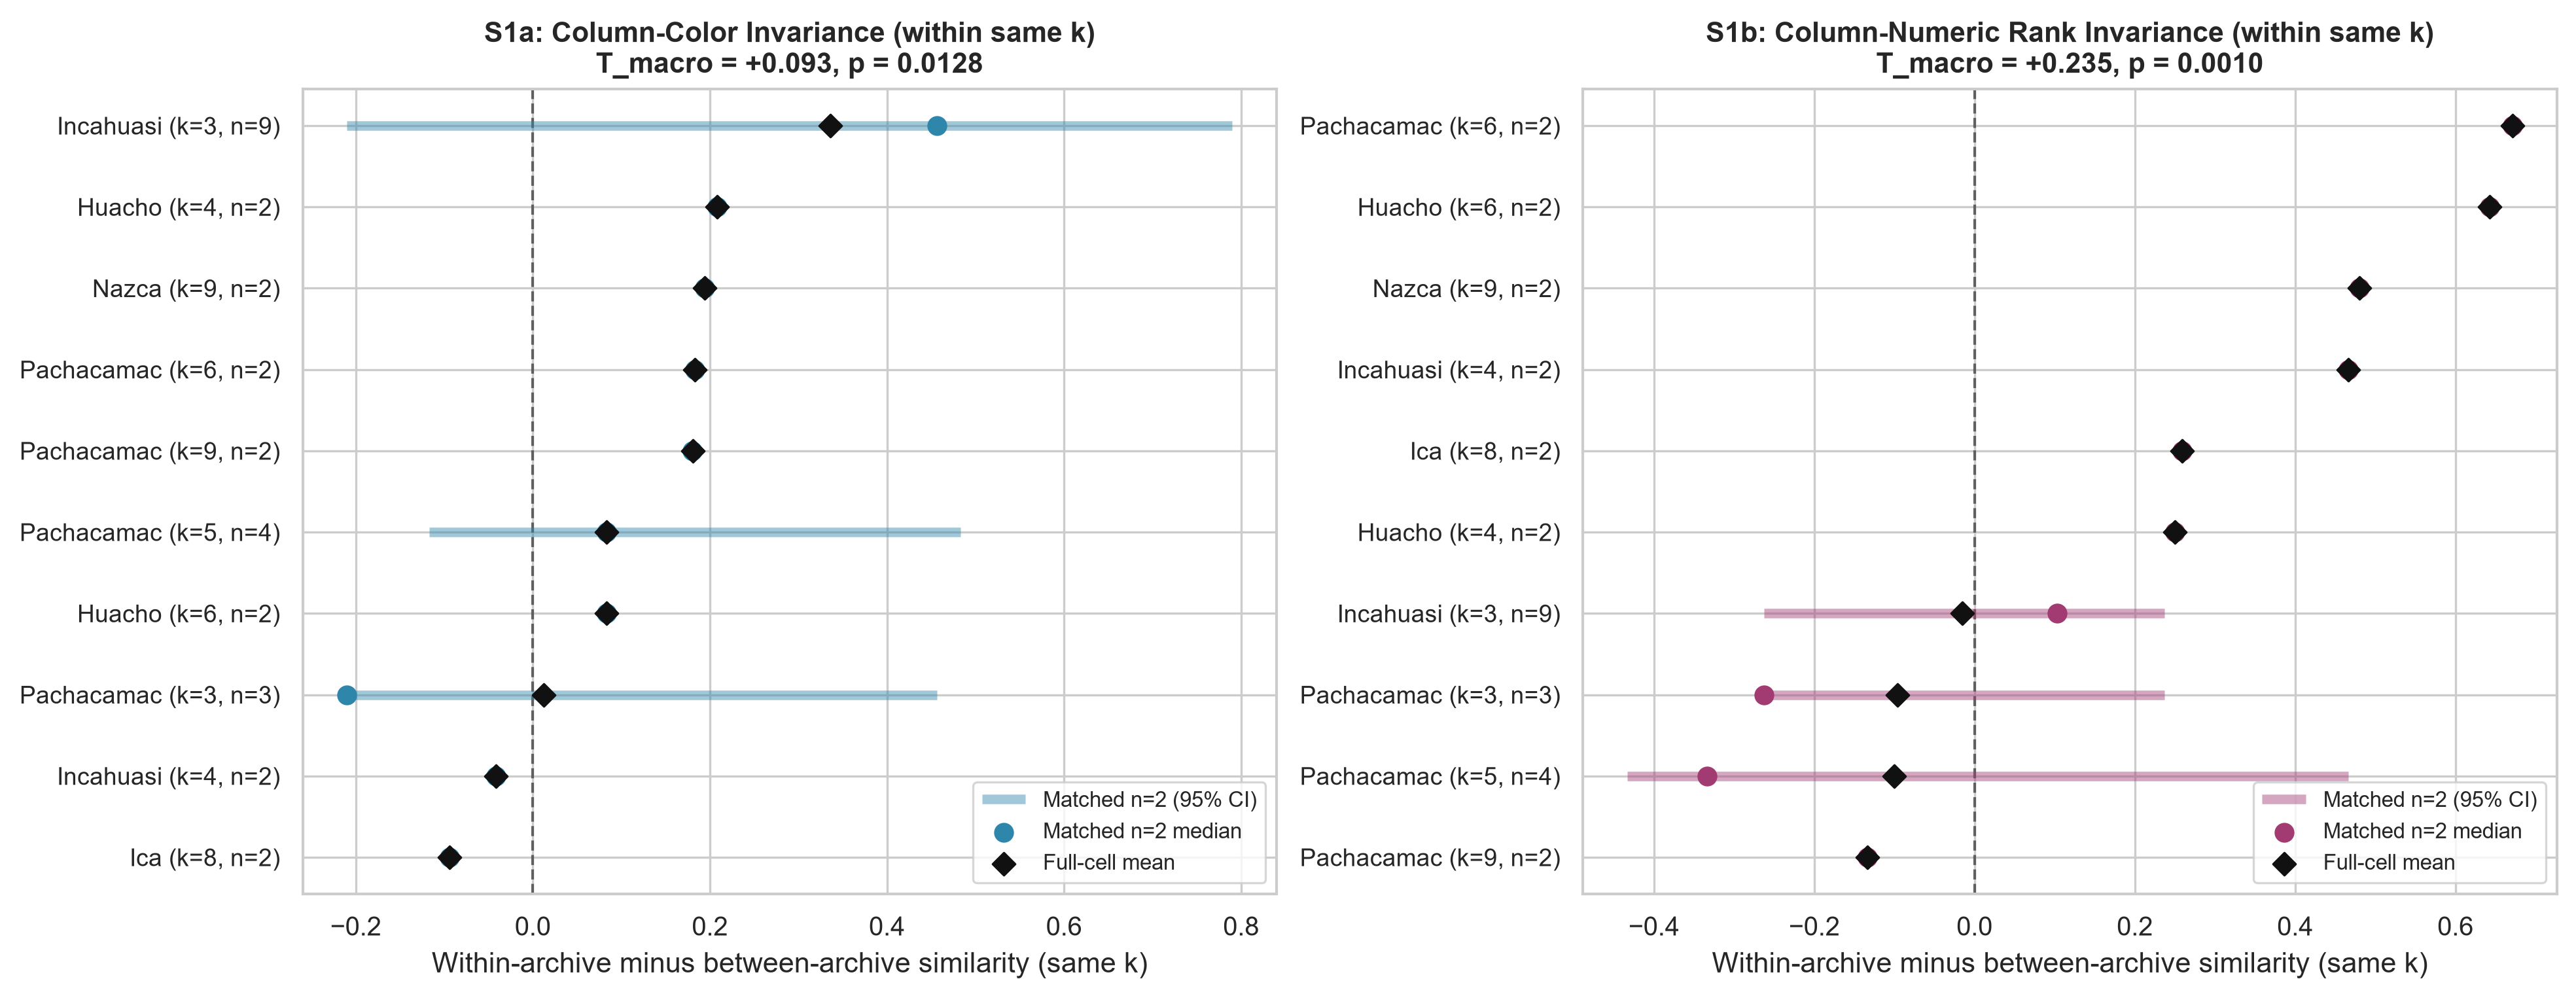
\includegraphics[width=\textwidth]{../figures/fig1_step1_archive_invariance.png}
  \caption{\textbf{\texttt{[PREREG]} Inter-archive invariance controlling for column count $k$ and archive sample size (Step 1).} Within-archive minus between-archive column similarity across $10$ $(site, k)$ cells ($n=44$ provenienced specimens from \texttt{primary\_86}) for color (\textbf{left}, S1a) and numeric column rank (\textbf{right}, S1b).}
  \label{fig:step1}
\end{figure}

In Step~2, $21/86$ ($24.4\%$) specimens fall outside all four deterministic structural families (individual dossiers in \texttt{results/step2\_outliers\_dossier.csv}), while unsupervised HDBSCAN leaves $45/86$ ($52.3\%$) as unforced noise (Fig.~\ref{fig:step2}). Post-hoc Fisher tests (\texttt{[EXPLORATORY]}; Fig.~\ref{fig:sub_step2}) indicate that deterministic \texttt{OUT} captures official calendar khipus ($\mathrm{OR} = 10.67$, $p = 0.0435$) and KFG Part~B paired khipus ($\mathrm{OR} = 7.41$, $p = 0.0294$), whereas HDBSCAN noise shows no enrichment ($\mathrm{OR} = 0.29\text{--}0.43$, $p > 0.34$).

\begin{figure}[t]
  \centering
  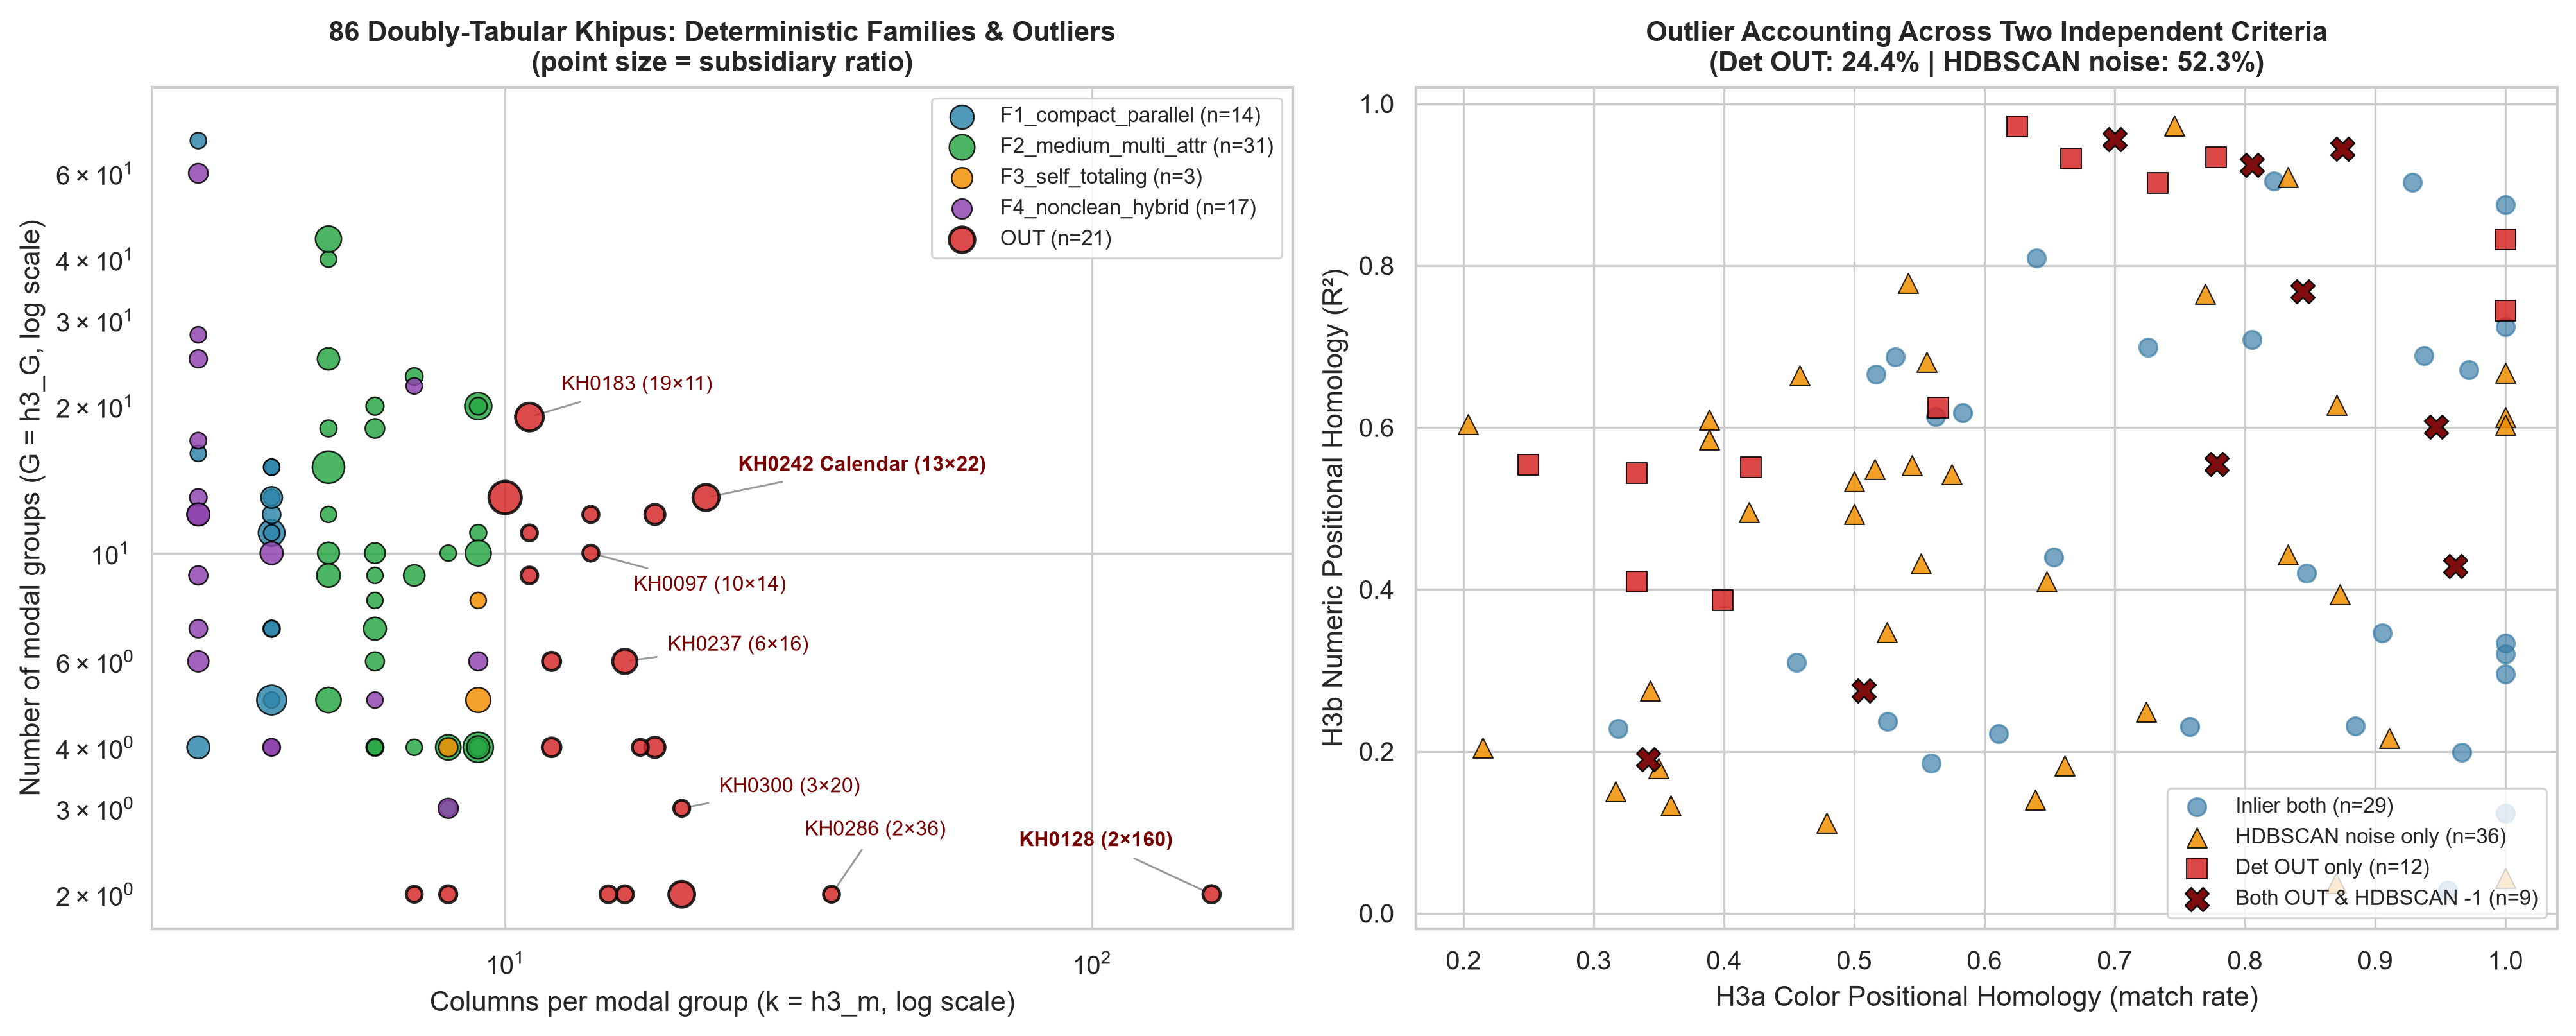
\includegraphics[width=\textwidth]{../figures/fig2_step2_taxonomy_outliers.png}
  \caption{\textbf{\texttt{[PREREG]} Structural taxonomy and dual outlier accounting across the $86$ doubly-tabular khipus (Step 2).} \textbf{Left:} Group-by-column geometry ($G \times k$) highlighting deterministic outliers (\texttt{OUT}, $21/86$). \textbf{Right:} Cross-tabulation of \texttt{OUT} against HDBSCAN unforced noise ($45/86$).}
  \label{fig:step2}
\end{figure}

\begin{figure}[t]
  \centering
  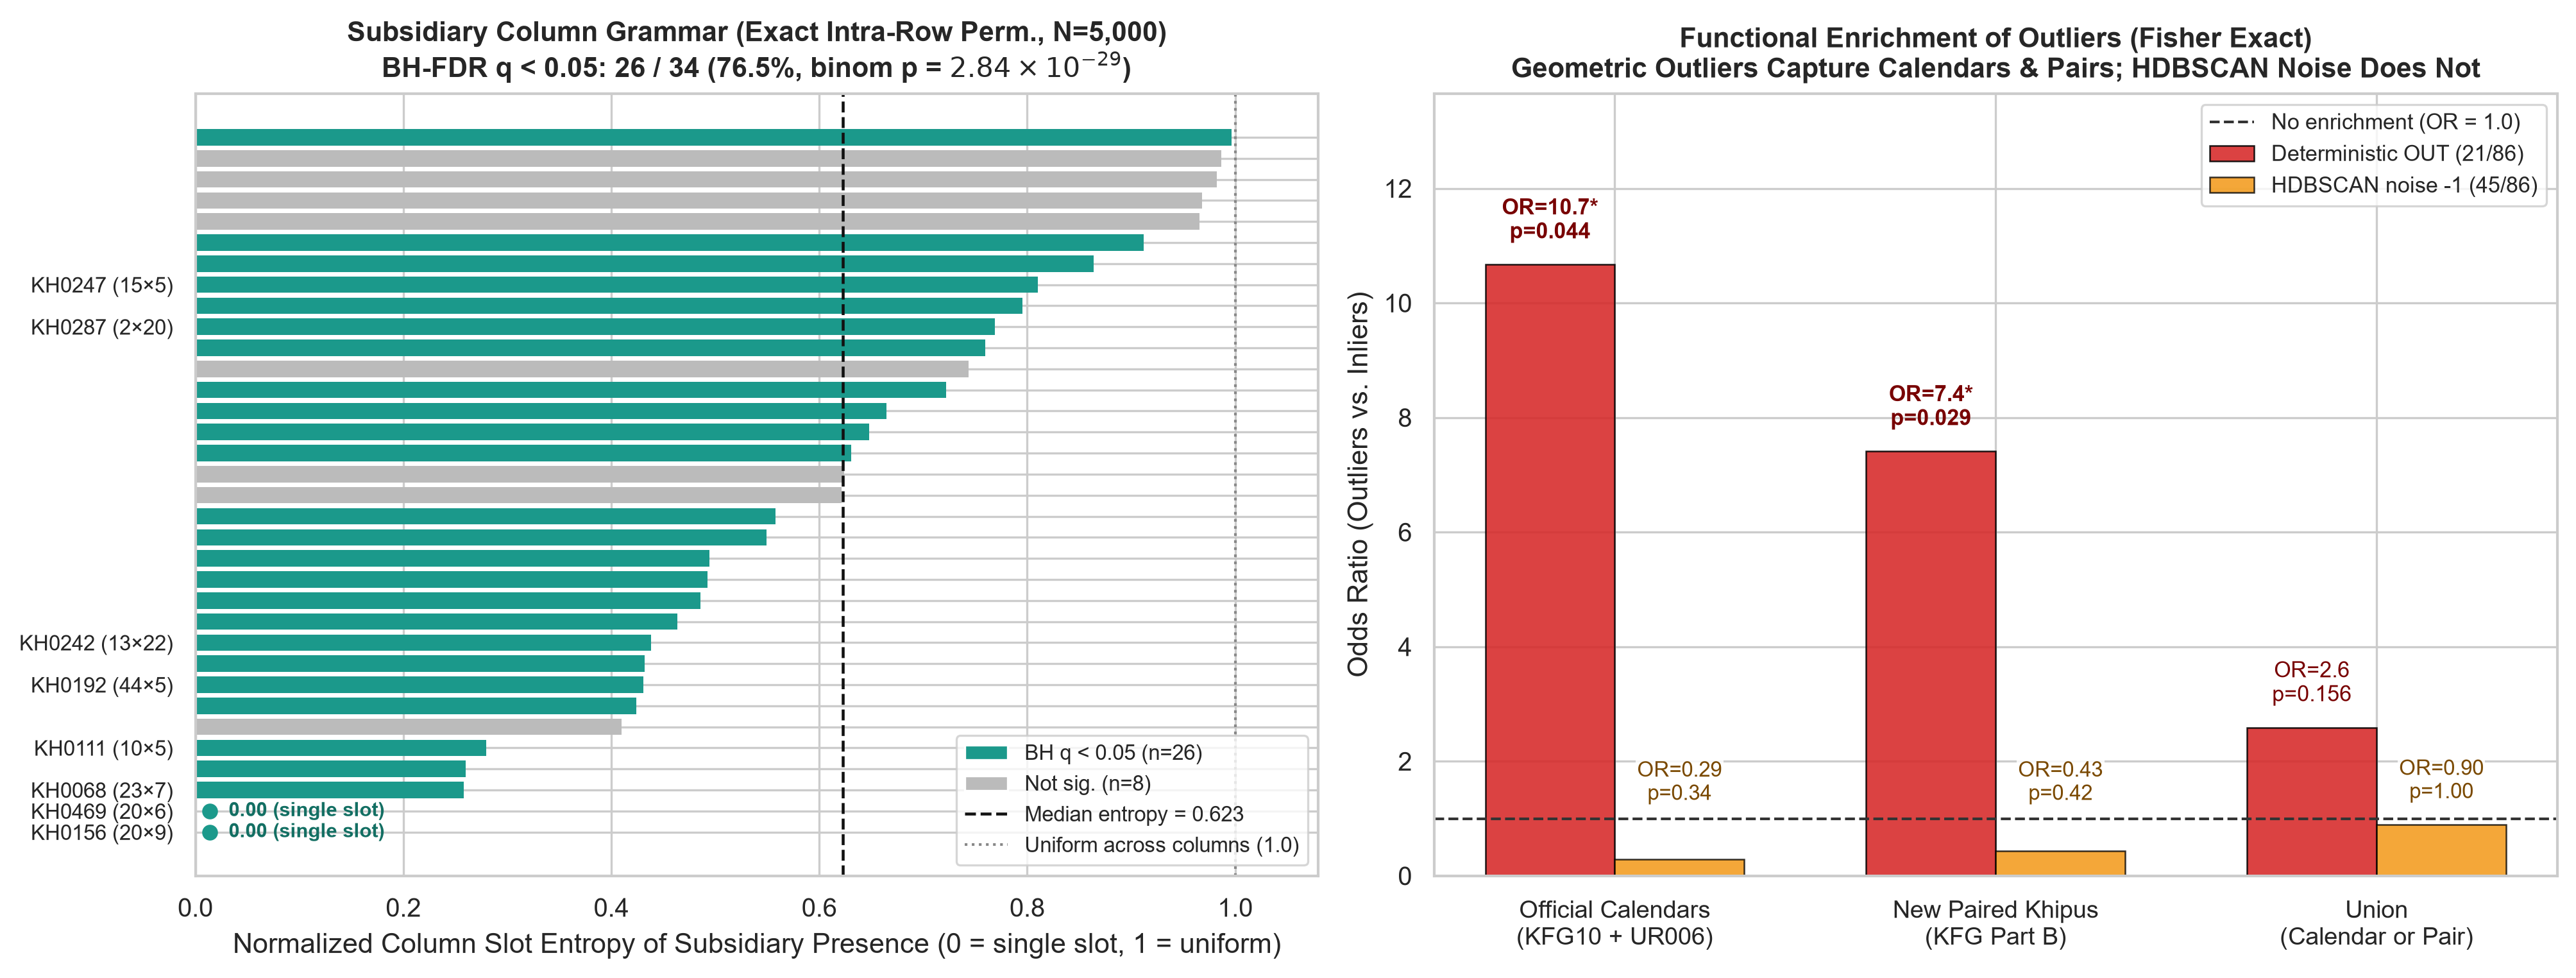
\includegraphics[width=\textwidth]{../figures/fig3_subsidiary_grammar_outliers.png}
  \caption{\textbf{\texttt{[EXPLORATORY]} Step 2 hardening: exact intra-row subsidiary slot permutation ($26/34 = 76.5\%$ BH-FDR) and Fisher enrichment of deterministic \texttt{OUT} versus HDBSCAN noise.}}
  \label{fig:sub_step2}
\end{figure}

\subsection{Five Candidate Hierarchical Subsidiary Regularities (Phase 2A, \texttt{[EXPLORATORY]})}

Correcting KFG \texttt{khipu\_summary.csv}'s $2{,}313$-cord drop by tracing all \texttt{CORD\_LEVEL >= 2} cords directly in \texttt{khipu.db} ($403$ khipus, $15{,}302$ parent-matched subsidiaries) and removing $9$ duplicate/paired specimens (Berlin, Huacho, Nazca, Huaquerones, Puruchuco, and Inkawasi pairs), we evaluate five candidate regularities at the **khipu level** (Table~\ref{tab:5reg}, Fig.~\ref{fig:phase2a}) and test blind out-of-sample replication on $36$ strictly disjoint KFG-only workbooks ($27$ with subsidiaries, $605$ cords). Because these five regularities were selected post hoc after exploring the corpus, Holm--Bonferroni and BH adjustment across the five reported tests ($p_{\mathrm{Holm}} \le 2.12 \times 10^{-3}$) controls only the reported family and underestimates broader exploratory multiplicity; blind KFG OOS replication therefore serves as the primary guard against overfitting.

\begin{enumerate}
  \item \textbf{R1 (Slot-locked attachment):} $39/83$ ($47.0\%$, Wilson $95\%$ CI $36.6\text{--}57.6\%$) of deduplicated multi-group OKR khipus pass individual intra-row permutation BH-FDR ($N_{\mathrm{perm}} = 2{,}000$, $p_{\min} = 1/2001$; exact binomial vs.\ $5\%$: $p = 1.47 \times 10^{-28}$, $p_{\mathrm{Holm}} = 7.35 \times 10^{-28}$). Blind KFG OOS: $5/6$ ($83.3\%$, $p = 1.80 \times 10^{-6}$).
  \item \textbf{R2 (Fourth-axis subsidiary color, strict $\text{sub} \neq \text{parent}$):} Although $80.3\%$ of OKR subsidiaries ($83.0\%$ KFG OOS) differ in color from their host cord, excluding parent-color copies still yields $44/65$ positive khipus (median $+3.69\text{ pp}$, bootstrap $95\%$ CI $+0.72$ to $+7.67\text{ pp}$; rank-biserial $r_{\mathrm{rb}} = +0.635$, $Z = +4.35$, asymptotic Wilcoxon $p = 1.36 \times 10^{-5}$, $p_{\mathrm{Holm}} = 4.08 \times 10^{-5}$).
  \item \textbf{R3 (Fifth-axis subsidiary numeric homology):} $41/73$ positive excess $R^2$ (median $+5.13\text{ pp}$, bootstrap $95\%$ CI $-2.02$ to $+11.67\text{ pp}$, which \emph{includes zero}; $r_{\mathrm{rb}} = +0.428$, $Z = +3.18$, Wilcoxon $p = 1.47 \times 10^{-3}$, $p_{\mathrm{Holm}} = 2.12 \times 10^{-3}$; KFG OOS $5/5$ positive). Given the wide median CI spanning zero, R3 represents a modest, heterogeneous candidate signal rather than a uniform rule.
  \item \textbf{R4 (Recursive decay, monotonic scaling, and part-whole sums):} At the khipu level ($n = 363$ deduplicated khipus, $7{,}971$ $L_1 \to L_2$ pairs), median fraction $\text{child} < \text{parent}$ is $77.8\%$ ($95\%$ CI $70.0\text{--}81.0\%$, $r_{\mathrm{rb}} = +0.561$, $Z = +8.93$, $p = 2.41 \times 10^{-19}$, $p_{\mathrm{Holm}} = 9.64 \times 10^{-19}$; pair-level $71.6\%$, $r_{\mathrm{rb}} = -0.633$, $Z = -46.6$, asymptotic $p < 10^{-300}$; KFG OOS $72.4\%$, $p = 1.15 \times 10^{-32}$). Non-trivial exact part-whole sums ($\sum \text{subs} = \text{parent} \ge 10$, $\ge 2$ knotted subs) occur $24$ times vs.\ $9.92$ null ($2.42\times$ enrichment, permutation $p = 0.0002$ at $N_{\mathrm{perm}} = 5{,}000$, $p_{\min} = 1/5001$).
  \item \textbf{R5 (Physical vertical spacing dose-response):} Evaluated conservatively at the \textbf{khipu level} to avoid treating clustered sibling pairs as independent, $84/137$ deduplicated khipus show $>50\%$ higher-over-lower descending sibling order (median $64.7\%$, Wilcoxon $p = 1.06 \times 10^{-3}$, $p_{\mathrm{Holm}} = 2.12 \times 10^{-3}$; replicated across $6$ catalogers). Descriptively at the pair level, descending order rises monotonically from $46.7\%$ at the $\Delta\text{AP} = 0\text{ cm}$ negative control ($n = 4{,}951$) to $65.1\%$ ($95\%$ CI $62.2\text{--}67.9\%$, $697/1{,}070$ pairs, $\Delta = +18.5\text{ pp}$) at $\Delta\text{AP} \ge 3\text{ cm}$ (Fig.~\ref{fig:phase2a}C). An apparent $R \to V$ attachment flip was traced to a single cataloger ($1{,}041/1{,}390$ pairs) and rejected.
\end{enumerate}

Across eight major archaeological sites (Fig.~\ref{fig:phase2a}D), exact-mirror entries ($\text{sub} = \text{parent}$) vary substantially ($\chi^2 = 191.3$, $p = 8.12 \times 10^{-38}$: Inkawasi $19.8\%$ and Huacho $20.4\%$ vs.\ Nazca/Ica/Pachac{\'a}mac $5.6\text{--}5.7\%$), and khipu-level attachment height varies significantly (Kruskal--Wallis $H = 21.75$, $p = 0.0028$).

\begin{table}[t]
  \centering
  \caption{\textbf{\texttt{[EXPLORATORY]} Deduplicated khipu-level OKR effect sizes, Holm-adjusted $p$-values across the five post-hoc candidate regularities (underestimating broader exploratory multiplicity), and blind KFG-only OOS replication.}}
  \label{tab:5reg}
  \small
  \begin{tabular}{@{}p{3.8cm}p{5.0cm}ccp{3.1cm}@{}}
    \toprule
    \textbf{Candidate Regularity} & \textbf{Deduplicated OKR Effect (95\% CI)} & \textbf{Khipu $p$} & \textbf{Holm $p$} & \textbf{Blind KFG OOS} \\
    \midrule
    R1: Slot-locked ($39/83$) & $47.0\%$ ($36.6\text{--}57.6\%$) BH-sig & $1.47\times 10^{-28}$ & $7.35\times 10^{-28}$ & $5/6$ ($p=1.80\times 10^{-6}$) \\
    R2: 4th-axis color ($44/65$) & $+3.69$ pp ($+0.72$ to $+7.67$); $r_{\mathrm{rb}}=+0.635$ & $1.36\times 10^{-5}$ & $4.08\times 10^{-5}$ & $3/5$ pos., med $+18.1$ pp \\
    R3: 5th-axis value ($41/73$) & $+5.13$ pp ($-2.02$ to $+11.67$, incl.\ $0$); $r_{\mathrm{rb}}=+0.428$ & $1.47\times 10^{-3}$ & $2.12\times 10^{-3}$ & $5/5$ ($100\%$; \texttt{AS005} $p=0.019$) \\
    R4: Decay $L_1\to L_2$ ($363$ kh.) & Med $77.8\%$ ($70.0\text{--}81.0\%$); $r_{\mathrm{rb}}=+0.561$ & $2.41\times 10^{-19}$ & $9.64\times 10^{-19}$ & $72.4\%$ ($p=1.15\times 10^{-32}$) \\
    R5: Vertical ($84/137$ kh.) & Med $64.7\%$; pair $65.1\%$ ($\ge 3\text{ cm}$) vs.\ $46.7\%$ ($0\text{ cm}$) & $1.06\times 10^{-3}$ & $2.12\times 10^{-3}$ & No \texttt{ATTACH\_POS} in KFG \\
    \bottomrule
  \end{tabular}
\end{table}

\begin{figure}[t]
  \centering
  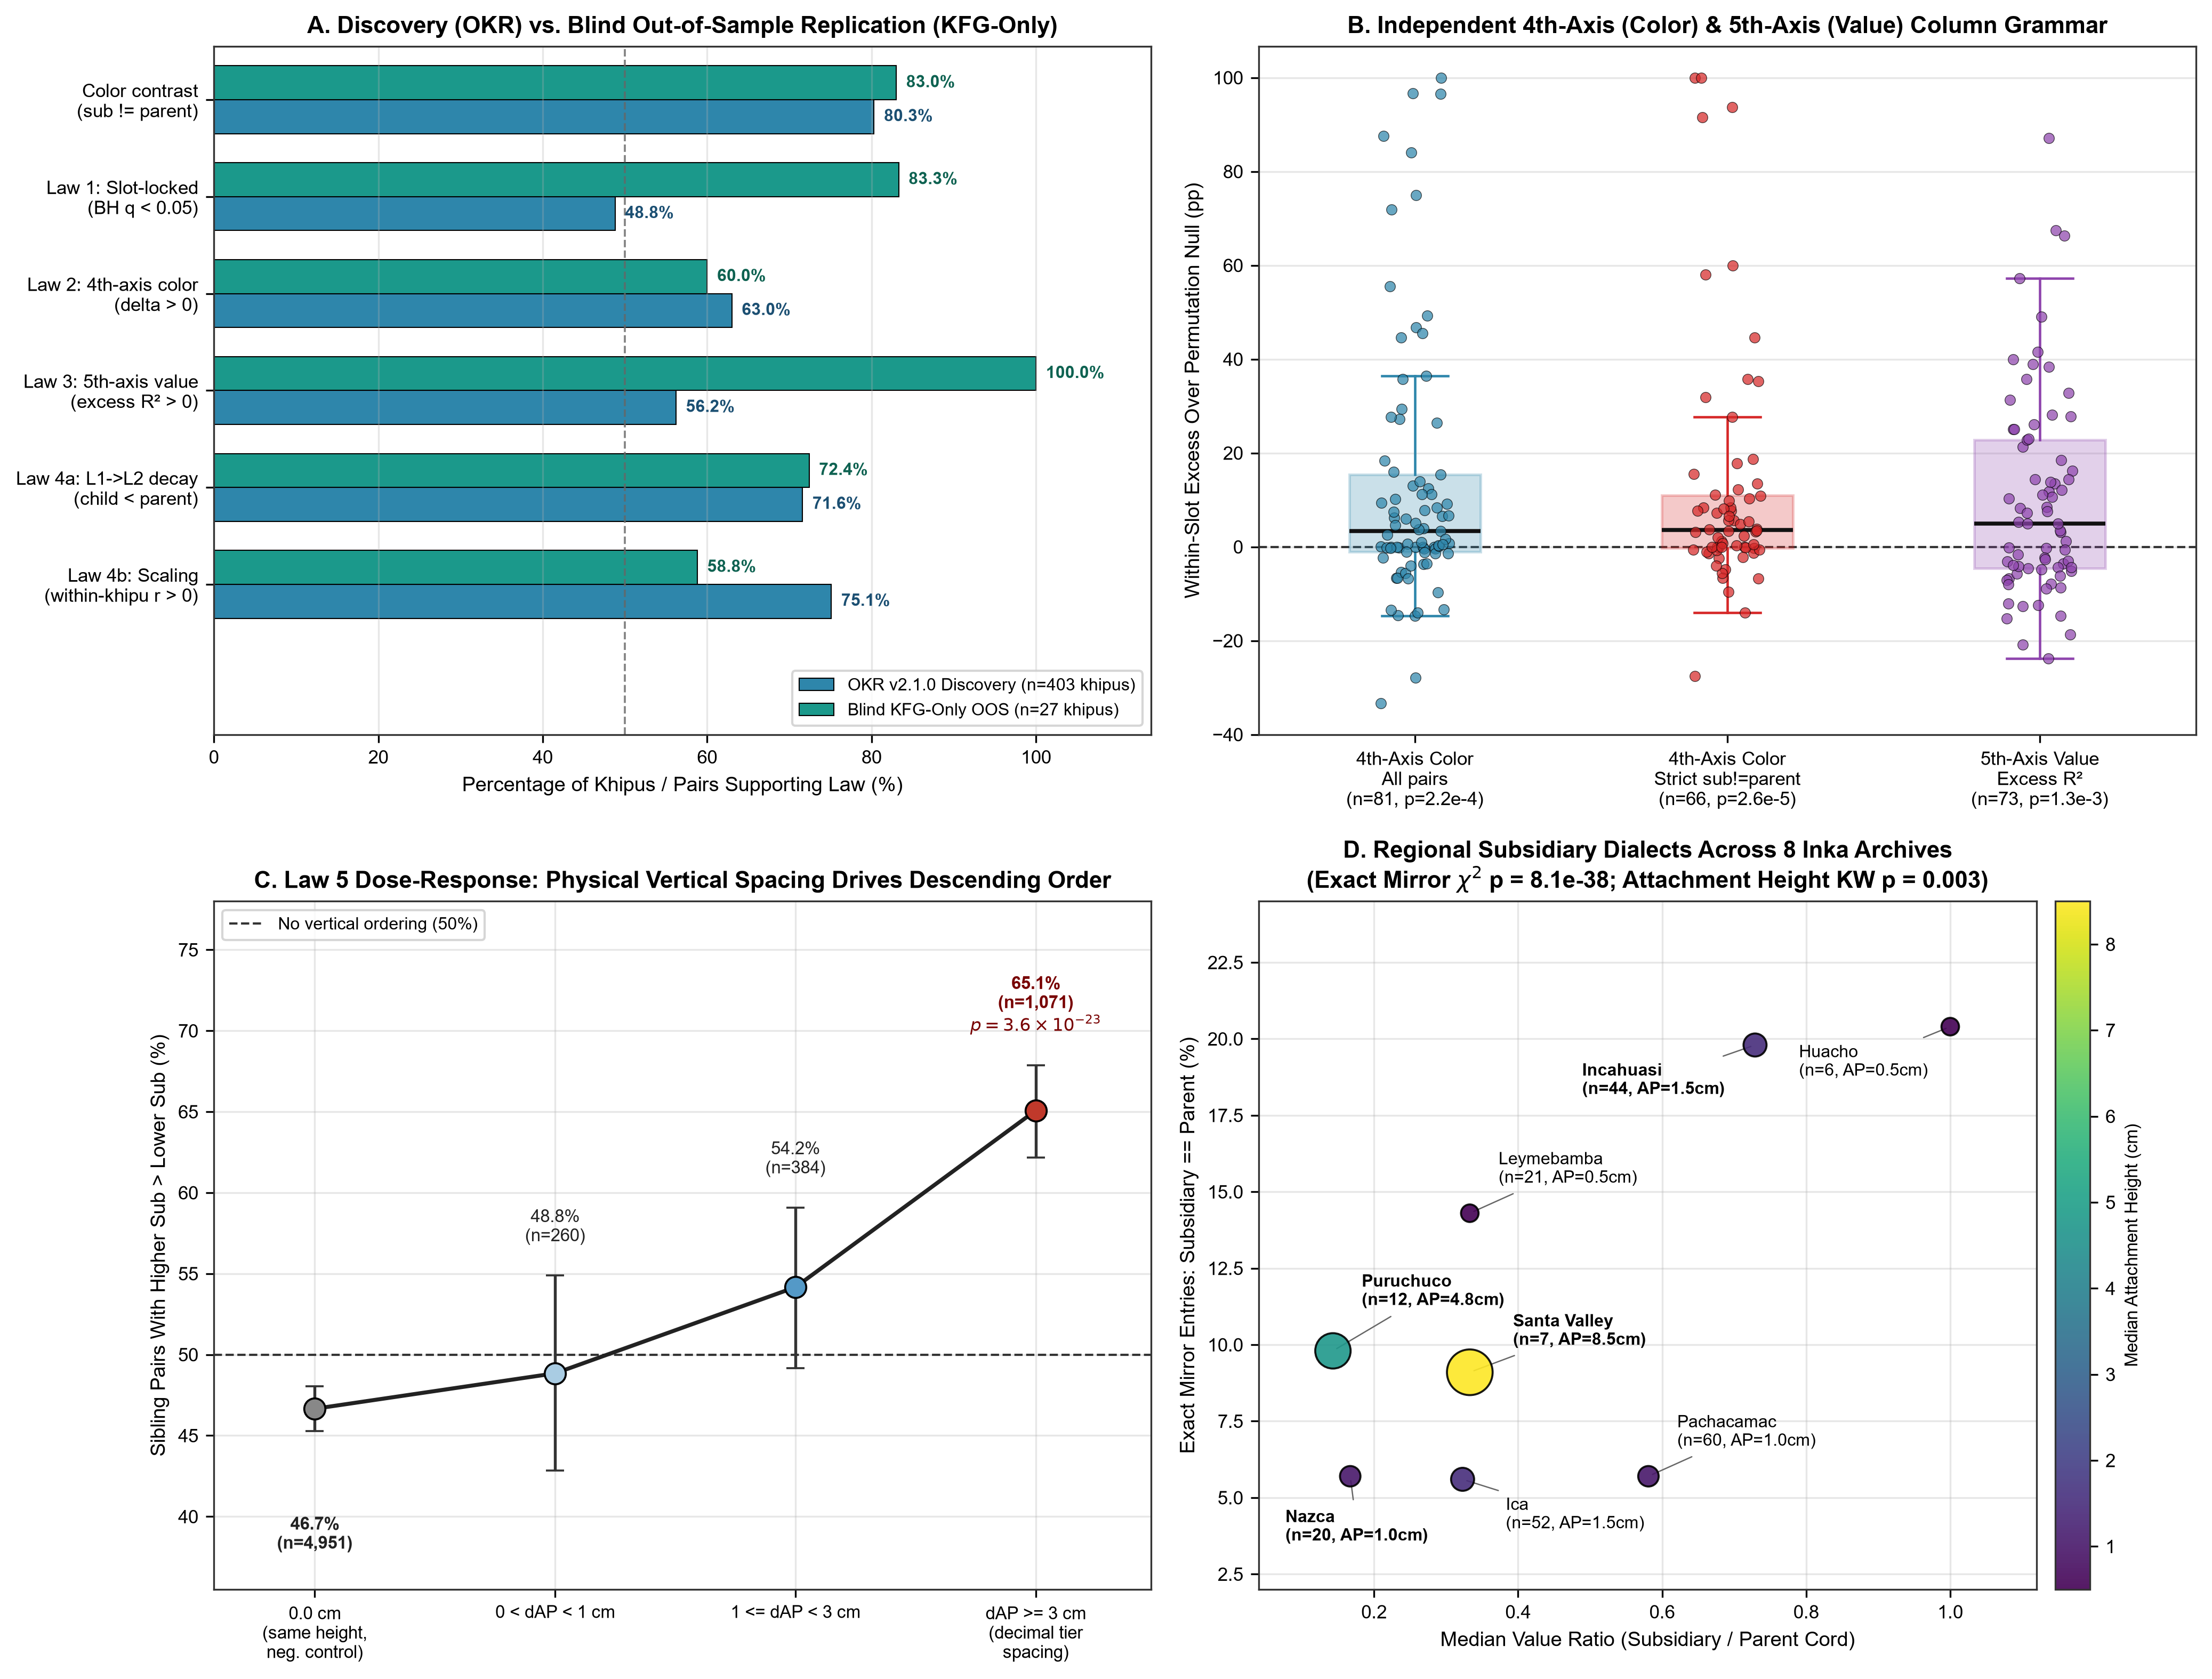
\includegraphics[width=\textwidth]{../figures/fig5_phase2a_candidate_regularities.png}
  \caption{\textbf{\texttt{[EXPLORATORY]} Five candidate subsidiary regularities, blind KFG OOS replication, $\Delta\text{AP}$ vertical dose-response negative control, and regional variation across eight archives (Phase 2A).}}
  \label{fig:phase2a}
\end{figure}

\subsection{Descriptive Corpus-Wide Pair Sweep: Putative Berlin Split-Ledger Triptych and Reversed Duplicate (Phase 2C, \texttt{[EXPLORATORY]})}

Across $611$ OKR v2.1.0 khipus ($\binom{611}{2} = 186{,}355$ possible pairs), \texttt{run\_corpus\_rare\_number\_sweep()} restricts to khipus with $\ge 5$ rare non-round values ($\ge 11$, non-multiples of $10$) and retains every pair passing the deterministic pre-filter $n_{\mathrm{rare,dist}} \ge 5$ and ($\text{Dice}_{\mathrm{rare}} \ge 0.25$ or $n_{\mathrm{rare,dist}} \ge 10$), yielding $538$ candidate pairs in \texttt{results/phase2c\_corpus\_pair\_sweep.csv} ranked by exact ordered rare-number matches across lags $[-10, +10]$. Because no sweep-wide multiple-testing correction is applied across the $\sim 186\text{k}$ pairs, all sweep findings are reported **descriptively via discovery rank**, and cell-shuffling $p \le 10^{-4}$ values are explicitly labeled as conditional post-selection permutations (a full-sweep empirical null calibration is deferred to the companion OKR$\leftrightarrow$KFG concordance study). The sweep recovers known controls ($\#2/538$ \texttt{AS125/UR247}, $\#7\text{--}8/538$ Inkawasi \texttt{UR255/UR267A} and \texttt{UR256/UR267B}, plus \texttt{UR066/UR067} and Puruchuco \texttt{UR064/UR068} \citealt{urton2005khipu}) and surfaces two putative unflagged Berlin museum links (\texttt{DUPLICATE\_FLAG = 0}; Table~\ref{tab:pairs}, Fig.~\ref{fig:phase2c}):

\begin{itemize}
  \item \textbf{Putative Berlin Split-Ledger Triptych (three physical pieces):} Ranked \textbf{$\#1/538$} in the sweep ($36$ ordered exact rare matches vs.\ $8$ for the highest background pair at $\#4/538$), Piece~1 master \texttt{KH0192} (\texttt{AS175/UR1175}, Berlin \texttt{VA 42518}, Pachac{\'a}mac, $45\times 5$, median length $65\text{ cm}$, $114$ subsidiaries; structured into Part~1 [Groups~1--21], Part~2 [Groups~22--24, an internal Part-3 column-sum bridge correlating at $r = 0.978\text{--}0.995$ with Part~3 set sums], and Part~3 [Groups~25--45]; \citealt{ascher1981code}) aligns with Piece~2 \texttt{KH0470} (\texttt{UR233}, \texttt{VA 63038 b}, Huacho, $k=6$ with a zero-valued spacer column, median length $40.0\text{ cm}$) across Part~1 on $88/104$ ($84.6\%$) exact cells ($r = 0.9823$, $\rho = 0.9795$, conditional post-selection permutation $p \le 1/10001 = 10^{-4}$; length Mann--Whitney $p = 6.21 \times 10^{-28}$). Targeted inspection of Berlin lot \texttt{VA 63038} (outside the $\pm 10$ sweep lag) identified Piece~3 \texttt{KH0469} (\texttt{UR232}, \texttt{VA 63038(B)}, Huacho, $k=6$ with zero spacer, median length $51.5\text{ cm}$), matching Part~3 on $73/105$ ($69.5\%$) exact cells ($r = 0.9446$, $\rho = 0.9565$, conditional post-selection $p \le 10^{-4}$; length Mann--Whitney $p = 1.20 \times 10^{-6}$). Direct sliding-window checks confirm that Part~2 (Groups~22--24) does \emph{not} appear in any khipu of lot \texttt{VA 63038} (\texttt{UR231}, \texttt{UR232}, or \texttt{UR233}; max $2/15$ matches). \emph{[Pending archival verification with Ethnologisches Museum Berlin and KFG editors.]}
  \item \textbf{Putative reversed physical duplicate (\texttt{KH0121} $\leftrightarrow$ \texttt{KH0473}):} Ranked \textbf{$\#3/538$} in the sweep ($9$ ordered exact rare matches, $\text{Dice}_{\mathrm{rare}} = 0.900$), reading \texttt{UR237} (\texttt{VA 66834}, unknown provenance) in reverse matches \texttt{UR1107} (\texttt{VA 24370(B)}, M{\'a}rquez) on $27/29$ ($93.1\%$) values ($\rho = 0.9332$) and individual cord lengths ($r = 0.9767$, median $|\Delta\text{len}| = 1.5\text{ cm}$; Fig.~\ref{fig:phase2c}D), suggesting the same physical Berlin specimen was cataloged twice in opposite directions and suggesting M{\'a}rquez provenance for \texttt{UR237}, subject to museum inventory verification.
\end{itemize}

\begin{table}[t]
  \centering
  \caption{\textbf{\texttt{[EXPLORATORY]} Putative Berlin collection links from the descriptive $611 \times 611$ rare-number sweep ($538$ filtered pairs, Phase 2C).}}
  \label{tab:pairs}
  \small
  \begin{tabular}{@{}p{3.9cm}ccccp{4.3cm}@{}}
    \toprule
    \textbf{Putative Link (Sweep Rank)} & \textbf{Cells} & \textbf{Exact} & \textbf{$r$ / $\rho$} & \textbf{Med.\ Len.\ (cm)} & \textbf{Interpretation (Pending Museum Check)} \\
    \midrule
    \texttt{UR1175} P1 $\leftrightarrow$ \texttt{UR233} ($\#1$) & $104$ & $88$ ($84.6\%$) & $0.982$ / $0.980$ & $65.0$ vs.\ $40.0$ ($p=6.2\times 10^{-28}$) & Putative distinct copy ($k{:}5\to 6$) \\
    \texttt{UR1175} P3 $\leftrightarrow$ \texttt{UR232} (lot) & $105$ & $73$ ($69.5\%$) & $0.945$ / $0.957$ & $63.0$ vs.\ $51.5$ ($p=1.2\times 10^{-6}$) & Putative distinct copy ($k{:}5\to 6$) \\
    \texttt{UR1107} $\leftrightarrow$ \texttt{UR237} ($\#3$, rev) & $29$ & $27$ ($93.1\%$) & $0.977^*$ / $0.933$ & $66.5$ vs.\ $66.2$ ($|\Delta|=1.5$) & Putative same artifact (M{\'a}rquez) \\
    \bottomrule
  \end{tabular}
  \vspace{2pt}
  {\footnotesize $^*$Cord-length Pearson $r = 0.977$; reversed value Spearman $\rho = 0.933$. Cell-shuffling $p \le 10^{-4}$ values for Parts~1 and 3 are conditional post-selection permutations without sweep-wide multiplicity correction.}
\end{table}

\begin{figure}[t]
  \centering
  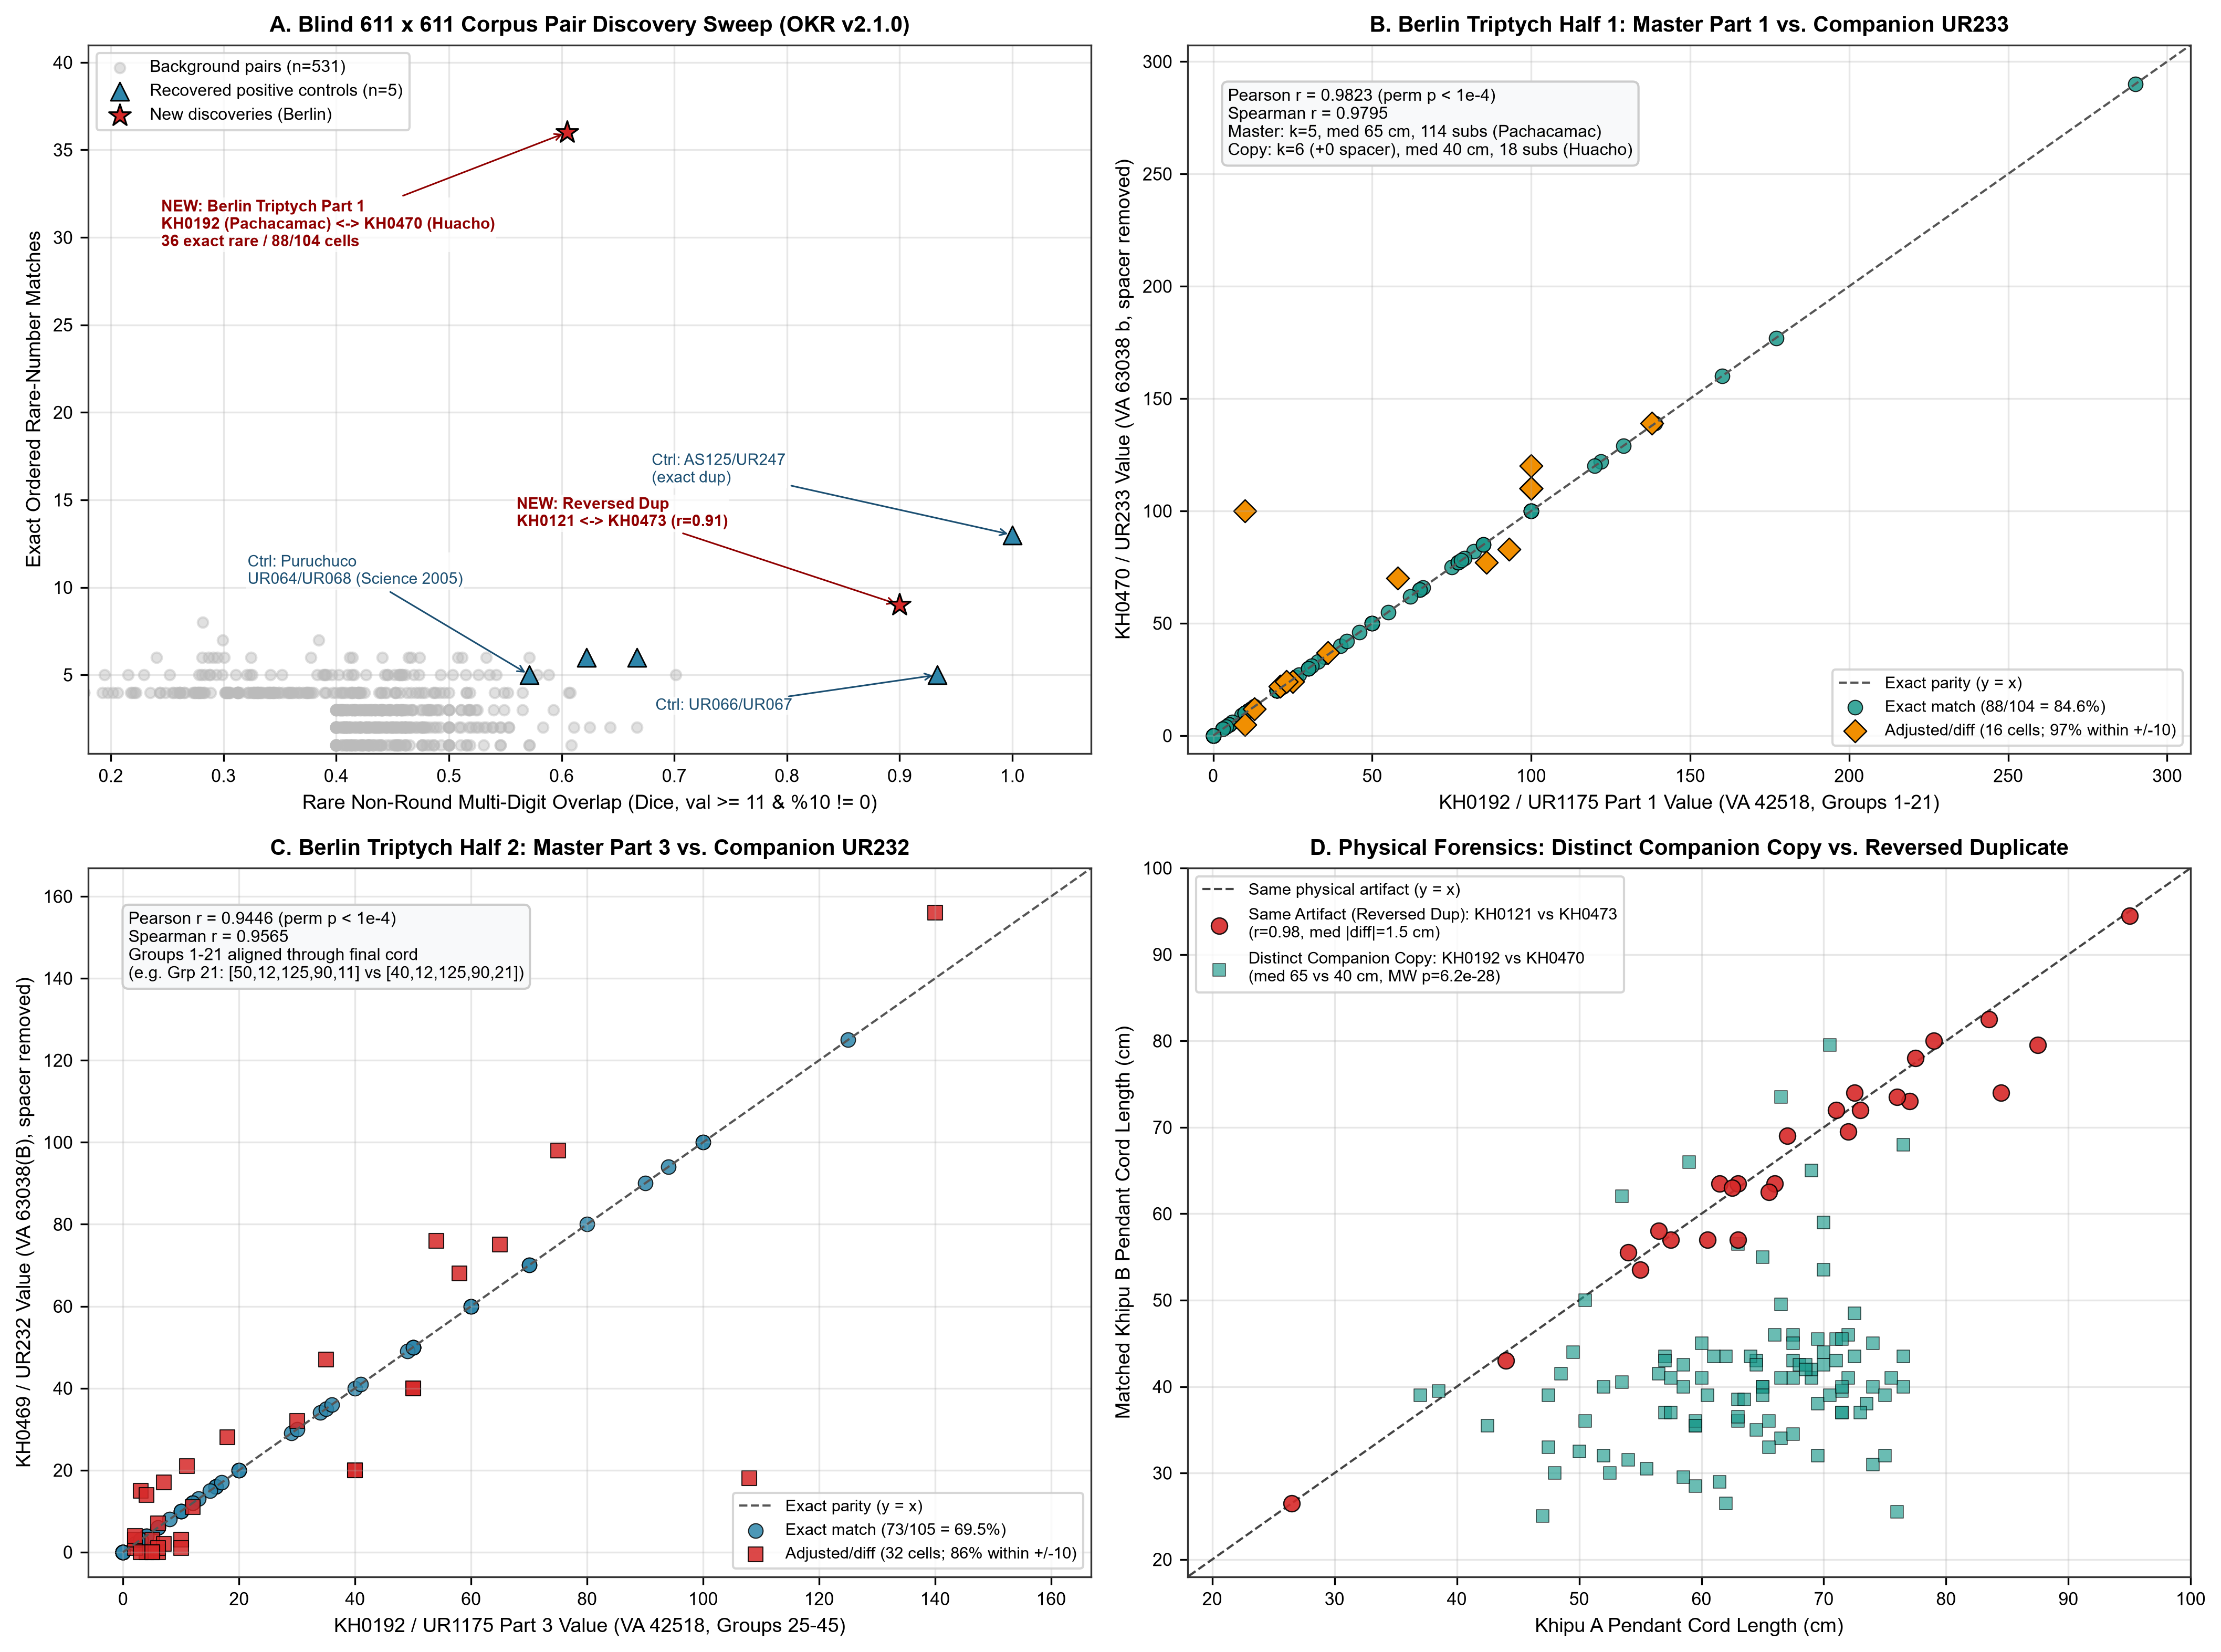
\includegraphics[width=\textwidth]{../figures/fig6_phase2c_berlin_triptych_and_pairs.png}
  \caption{\textbf{\texttt{[EXPLORATORY]} Descriptive corpus-wide $611 \times 611$ sweep ($538$ filtered pairs), putative Berlin split-ledger triptych, and physical cord-length forensics (Phase 2C).}}
  \label{fig:phase2c}
\end{figure}

\subsection{Proxy Calibration, Pre-Specified Alignment Null, and Power Analysis (Gate 0 \& Step 3)}

As documented in \texttt{DEVIATIONS.md}, the pre-specified Santa Valley 1670 khipu-to-text positive control proved structurally infeasible (the 1670 revisita lacks a 6-column table) and was replaced by Gate~0A structural replication of \citet{medrano2018toward} ($133/133$ groups, $63\text{R}/69\text{V}$, first-cord sum $369$ vs.\ $367$ pesos) and Gate~0B proxy controls ($A_{\mathrm{JSD}} = 0.977\text{--}0.985$, Null~2 $p = 0.0002$ across Santa Valley $k=6$ pairs; Huaraz 1532$\leftrightarrow$1558 $A_{\mathrm{JSD}} = 0.9774$, Null~1 $p = 0.00952$; Fig.~\ref{fig:step3}).

Against five verbatim highland \emph{Textos Andinos} schemas (note that the three Huaraz schemas are non-independent, representing three effective archival traditions: Chucuito, Huaraz, Sacaca), Step~3 yields \textbf{$0/30$} BH-FDR hits in \texttt{primary\_86} and \textbf{$0/22$} in \texttt{sens\_H3b\_only} under exact arity, and \textbf{$0/70$} in \texttt{primary\_86} under the secondary $|k_K - k_D| = 1$ sensitivity ($1/59$ in \texttt{sens\_H3b\_only}, \texttt{KH0278} Lima vs.\ Chucuito, failing Null~1 $p = 0.100$ and provenance). Noise-perturbation power simulations (\texttt{results/step3\_power\_analysis.csv}) quantify power under both the nominal threshold ($p_{\mathrm{eval}} < 0.05$: $96.7\text{--}100\%$ up to $\sigma = 0.20$ and $71.7\text{--}84.2\%$ at $\sigma = 0.50$) and the actual **BH-FDR ($m=30$) decision rule**: at $\sigma = 0.20$, FDR power is **$70.8\%$ for $k=5$**, **$59.2\%$ for $k=7$**, and **$0\%$ for an isolated $k=6$ hit** due to Null~1's discreteness floor ($2/720 = 0.00278$, yielding $30 \times 0.00278 = 0.0833 > 0.05$ even at $\sigma = 0$, though no $k=6$ pair in \texttt{primary\_86} reached $p < 0.05$ or $A_{\mathrm{JSD}} \ge 0.97$).

\begin{figure}[t]
  \centering
  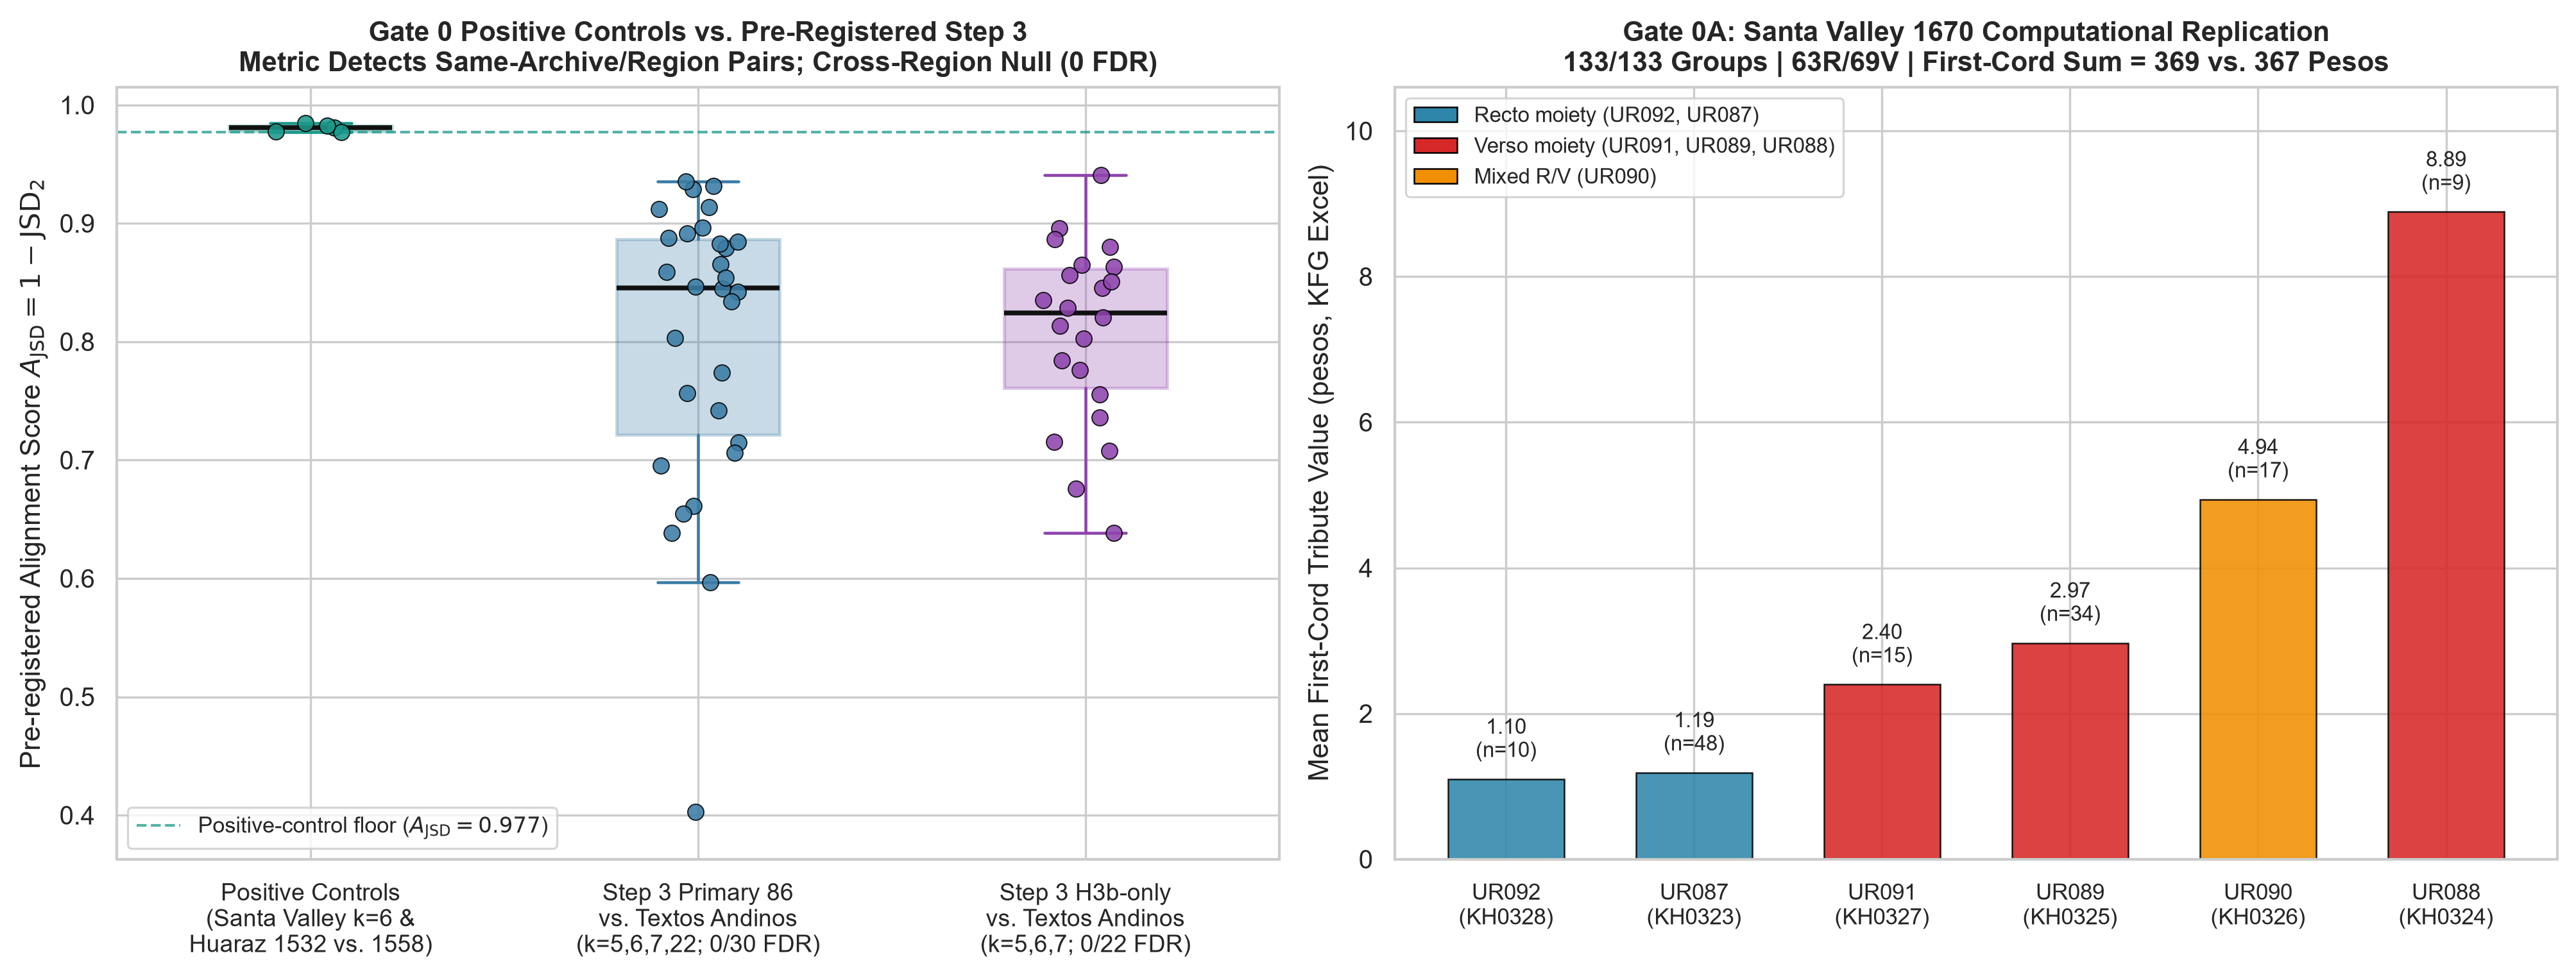
\includegraphics[width=\textwidth]{../figures/fig4_gate0_vs_step3_alignment.png}
  \caption{\textbf{Proxy positive controls (Gate 0) versus pre-specified cross-region alignment null (Step 3).}}
  \label{fig:step3}
\end{figure}

\section{Discussion and Limitations}

Our combined internally pre-specified and exploratory evidence motivates a concrete working hypothesis: surviving decimal tabular khipus implement a standardized multi-axis relational syntax (including candidate subsidiary regularities and putative split-ledger transcription conventions), whereas semantic cross-modal alignment is currently limited by the geographic mismatch between predominantly coastal surviving khipus and digitized highland colonial texts. Testing provenance-matched coastal colonial \emph{visitas} under an externally time-locked pre-registration protocol is the highest-leverage next step. In accordance with Step~4, non-decimal/anomalous specimens (\texttt{clean\_dec\_frac < 1.0}) and S/Z calendar candidates \citep{hyland2017writing,clindaniel2019toward,salomon2004cord} are excluded from decoding claims and reserved for future work.

\section{Methods}

Cord, knot, color, and provenance tables were extracted from OKR v2.1.0 (\texttt{khipu.db}; \citealt{okr2025v210}) and verified against $651$ individual KFG Excel workbooks (\texttt{KFG\_DB\_Excel/*.xlsx}; \citealt{khosla2024kfg}), avoiding KFG's \texttt{khipu\_summary.csv} due to its $2{,}313$-subsidiary drop. All code runs reproducibly via \texttt{uv run python -m src.<module>} with pinned dependencies (\texttt{uv.lock}), deterministic seeds, and $16$ automated \texttt{pytest} checks (CI-verified via GitHub Actions). Permutation tests report exact $p = (k+1)/(N_{\mathrm{perm}}+1)$ bounds; asymptotic tests accompany $p$-values with standardized effect sizes and $95\%$ confidence intervals; multiplicity is controlled via Benjamini--Hochberg FDR \citep{benjamini1995controlling} and Holm--Bonferroni. Raw third-party datasets (OKR v2.1.0, pinned KFG commit \texttt{167b8df}, and \emph{Textos Andinos} recitations) are excluded from Git and fetched locally with checksum verification via \texttt{scripts/fetch\_data.sh}. Code is licensed under MIT and repository-authored derived outputs under CC-BY-4.0 (excluding \texttt{data/colonial\_schemas/*.json}, which are listed separately as derived numerical matrices pending written permission from copyright holders; see \texttt{DATA\_LICENSE.md}) at \url{https://github.com/Disentangle-Lab/khipu-semantic-alignment} (archival Zenodo Concept DOI: \url{https://doi.org/10.5281/zenodo.24610674}).

\bibliographystyle{plainnat}
\bibliography{references}

\end{document}
